\section{比较量与收敛}
\label{sec:dcomp-convergence}

设$P_1,P_2,\dots$与$P$是一列分布，某个比较量$\rho(P_n,P)$趋于零。这能推出什么？能否推出另一个比较量也趋于零，能否推出第~\ref{chap:weak-convergence-of-distributions}章的弱收敛，矩是否也跟着收敛？本节逐一回答。弱收敛的定义与判别沿用那一章：$P_n\xrightarrow{\mathrm{w}}P$指对每个有界连续函数$f$，$\int f\,\mathrm{d}P_n\to\int f\,\mathrm{d}P$。那一章在$\mathbb{R}^{d}$上陈述；在一般度量空间上，定义只需把$\mathbb{R}^{d}$换成该空间，Portmanteau定理中“有界Lipschitz函数的期望收敛即可”这一判据的证明不变。

\subsection{散度与总变差的控制}
\label{sec:dcomp-pinsker}

先比较本身。总变差是最常用的标尺，KL散度和Hellinger距离与它有什么数量关系？本小节的对数一律取自然对数，总变差按定义~\ref{def:dcomp-tv}的约定，系数改变时下面的常数要相应改变。

\begin{theorem}[Pinsker不等式]
\label{thm:dcomp-pinsker}
对任意概率分布$P,Q$，
\begin{equation}
 d_{\mathrm{TV}}(P,Q)\leq\sqrt{\tfrac12D_{\mathrm{KL}}(P\Vert Q)} .
 \label{eq:dcomp-pinsker}
\end{equation}
\end{theorem}

\begin{proof}
\emph{化为两点分布。}若KL散度为$+\infty$，结论成立。设它有限，取$A^{*}=\{p>q\}$，用确定映射$x\mapsto\mathbf{1}_{A^{*}}(x)$把两个分布变成$\{0,1\}$上的两点分布$\operatorname{Bern}(a)$与$\operatorname{Bern}(b)$，其中$a=P(A^{*})$，$b=Q(A^{*})$。由定理~\ref{thm:dcomp-tv-density}，$d_{\mathrm{TV}}(P,Q)=a-b$；由定理~\ref{thm:dcomp-data-processing}，KL散度在映射后不增。所以只需证明两点分布的不等式
\[
 h(b)=a\ln\frac{a}{b}+(1-a)\ln\frac{1-a}{1-b}-2(a-b)^{2}\geq0,\qquad 0<b<1 .
\]

\emph{两点分布的情形。}固定$a\in[0,1]$，把$h$看成$b$的函数。$h(a)=0$。求导，
\[
 h'(b)=-\frac{a}{b}+\frac{1-a}{1-b}+4(a-b)=(b-a)\Bigl(\frac{1}{b(1-b)}-4\Bigr) .
\]
$b(1-b)\leq\tfrac14$，括号内非负，所以$h'(b)$与$b-a$同号：$h$在$b<a$时下降，在$b>a$时上升，最小值是$h(a)=0$。于是
\[
 D_{\mathrm{KL}}(P\Vert Q)\geq2(a-b)^{2}=2d_{\mathrm{TV}}^{2}(P,Q),
\]
开方即得。$b=0$或$1$而$a\neq b$时散度为$+\infty$，不需讨论。
\end{proof}

式~\eqref{eq:dcomp-pinsker}称为\term{Pinsker不等式}（Pinsker's inequality）。证明的思路值得留意：最坏事件$A^{*}$把一般分布压缩成一次是非判断，后处理不增加散度，于是一般情形归结为两点分布上的一元不等式。在例表上，$\sqrt{0.2773/2}\approx0.3723\geq0.3$。交换方向用$D_{\mathrm{KL}}(Q\Vert P)\approx0.3466$，得到$0.4163\geq0.3$，同样成立，因为总变差对称，任一方向的KL散度都控制它。图~\ref{fig:dcomp-pinsker}(a)在两点分布上比较两边：$P=\operatorname{Bern}(t)$，$Q=\operatorname{Bern}(\tfrac12)$，$t$接近$\tfrac12$时两条曲线几乎重合，常数$\tfrac12$不能再改进。

Pinsker不等式只有一个方向。总变差小不能推出KL散度小，甚至不能推出它有限。设$Q$在格点$0$处概率为零，例如$Q$是$\{1,2,\dots,10\}$上的均匀分布，令
\[
 P_\varepsilon=(1-\varepsilon)Q+\varepsilon\delta_0 .
\]
$P_\varepsilon$把$Q$的$\varepsilon$份质量挪到了点$0$，总变差是$\varepsilon$；但$P_\varepsilon(\{0\})=\varepsilon>0=Q(\{0\})$，$P_\varepsilon$不绝对连续于$Q$，$D_{\mathrm{KL}}(P_\varepsilon\Vert Q)=+\infty$。无论$\varepsilon$多小，总变差都看不出这个零概率格点上的冲突，KL散度则对它给出无穷大。

Hellinger距离与总变差之间是双向控制。

\begin{theorem}[Hellinger距离与总变差]
\label{thm:dcomp-hellinger-tv}
对任意概率分布$P,Q$，
\begin{equation}
 d_{\mathrm{H}}^{2}(P,Q)\leq d_{\mathrm{TV}}(P,Q)\leq d_{\mathrm{H}}(P,Q)\sqrt{2-d_{\mathrm{H}}^{2}(P,Q)} .
 \label{eq:dcomp-hellinger-tv}
\end{equation}
并且
\begin{equation}
 D_{\mathrm{KL}}(P\Vert Q)\geq2d_{\mathrm{H}}^{2}(P,Q) .
 \label{eq:dcomp-kl-hellinger}
\end{equation}
\end{theorem}

\begin{proof}
用共同支配测度写出密度。对每一点，
\[
 \lvert p-q\rvert=\lvert\sqrt{p}-\sqrt{q}\rvert\,(\sqrt{p}+\sqrt{q}),
\]
而右边第一个因子不超过第二个因子，所以$(\sqrt{p}-\sqrt{q})^{2}\leq\lvert p-q\rvert$。积分并乘以$\tfrac12$，得到左边的不等式。

对右边，用同一个分解与Cauchy--Schwarz不等式，
\[
 \frac12\int\lvert p-q\rvert\,\mathrm{d}\lambda\leq\frac12\Bigl(\int(\sqrt{p}-\sqrt{q})^{2}\,\mathrm{d}\lambda\Bigr)^{1/2}\Bigl(\int(\sqrt{p}+\sqrt{q})^{2}\,\mathrm{d}\lambda\Bigr)^{1/2} .
\]
第一个因子是$\sqrt2\,d_{\mathrm{H}}$；展开第二个因子中的平方，它是$(2+2B)^{1/2}$，由式~\eqref{eq:dcomp-hellinger-bc}，$B=1-d_{\mathrm{H}}^{2}$，所以第二个因子是$\sqrt2\,(2-d_{\mathrm{H}}^{2})^{1/2}$。代入即得右边的不等式。

最后，由定理~\ref{thm:dcomp-renyi-order}与式~\eqref{eq:dcomp-renyi-special}，$D_{\mathrm{KL}}\geq D_{1/2}=-2\ln B$，再由$-\ln B\geq1-B=d_{\mathrm{H}}^{2}$得式~\eqref{eq:dcomp-kl-hellinger}。
\end{proof}

在例表上，$d_{\mathrm{H}}^{2}\approx0.0757$，$d_{\mathrm{H}}\sqrt{2-d_{\mathrm{H}}^{2}}\approx0.3818$，总变差$0.3$确实夹在中间。式~\eqref{eq:dcomp-hellinger-tv}说明$d_{\mathrm{TV}}(P_n,P)\to0$当且仅当$d_{\mathrm{H}}(P_n,P)\to0$，两者定义的收敛相同，只是速度可能不同：一个是另一个的平方量级。图~\ref{fig:dcomp-pinsker}(b)在高斯平移族上画出这三条曲线以及Pinsker上界。

\begin{BookInlineFigure}
 \centering
 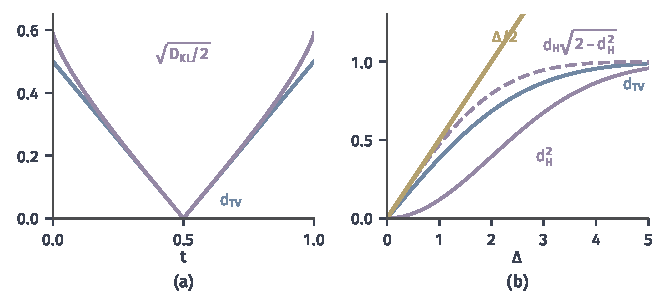
\includegraphics[width=112mm]{figures/07-probability/04-distribution-analysis/matplotlib/dcomp-pinsker/figure.pdf}
 \caption{散度对总变差的控制。(a)$P=\operatorname{Bern}(t)$，$Q=\operatorname{Bern}(\tfrac12)$：$d_{\mathrm{TV}}=\lvert t-\tfrac12\rvert$（蓝）与Pinsker上界$\sqrt{D_{\mathrm{KL}}(P\Vert Q)/2}$（紫）。(b)$P=\mathcal{N}(0,1)$，$Q=\mathcal{N}(\Delta,1)$：$d_{\mathrm{TV}}=2\Phi(\Delta/2)-1$（蓝），下界$d_{\mathrm{H}}^{2}=1-\mathrm{e}^{-\Delta^{2}/8}$（紫），上界$d_{\mathrm{H}}\sqrt{2-d_{\mathrm{H}}^{2}}$（紫色虚线），Pinsker上界$\Delta/2$（黄）。}
 \label{fig:dcomp-pinsker}
\end{BookInlineFigure}

\paragraph{总变差强于弱收敛}
若$d_{\mathrm{TV}}(P_n,P)\to0$，对每个有界连续$f$，由式~\eqref{eq:dcomp-tv-osc}，
\[
 \Bigl\lvert\int f\,\mathrm{d}P_n-\int f\,\mathrm{d}P\Bigr\rvert\leq2\lVert f\rVert_{\infty}\,d_{\mathrm{TV}}(P_n,P)\to0,
\]
所以$P_n\xrightarrow{\mathrm{w}}P$。反过来不成立。$\delta_{1/n}\xrightarrow{\mathrm{w}}\delta_0$，总变差却恒为$1$。一个更典型的例子是用离散分布逼近连续分布：令$U_n$是$n$个格点$(2k-1)/(2n)$（$k=1,\dots,n$）上的均匀分布，$U=\operatorname{Unif}(0,1)$。$U_n\xrightarrow{\mathrm{w}}U$，这是第~\ref{chap:weak-convergence-of-distributions}章Riemann和的例子（只把右端点换成中点）。但$U_n$集中在有限集上，那个集合的Lebesgue测度为零，两者相互奇异，$d_{\mathrm{TV}}(U_n,U)=1$，$D_{\mathrm{KL}}(U_n\Vert U)=+\infty$。

一阶Wasserstein距离却能正确地衡量这个逼近。把$(0,1)$分成$n$个长为$1/n$的小区间，每个格点恰在一个小区间的中点。把每个小区间里的均匀质量搬到它的中点，是一个耦合，平均搬运距离是
\[
 n\int_{0}^{1/n}\Bigl\lvert t-\frac{1}{2n}\Bigr\rvert\,\mathrm{d}t=\frac{1}{4n} .
\]
反过来，$g(x)=\min_k\lvert x-(2k-1)/(2n)\rvert$是到格点集合的距离，它是1-Lipschitz函数，在$U_n$下平均为$0$，在$U$下平均也是$1/(4n)$。由第~\ref{sec:dcomp-kr}节的上下界，$W_1(U_n,U)=1/(4n)$。图~\ref{fig:dcomp-lattice-metrics}比较三种量：总变差停在$1$，$W_1$按$1/n$下降，高斯核MMD下降得更快。

\begin{BookInlineFigure}
 \centering
 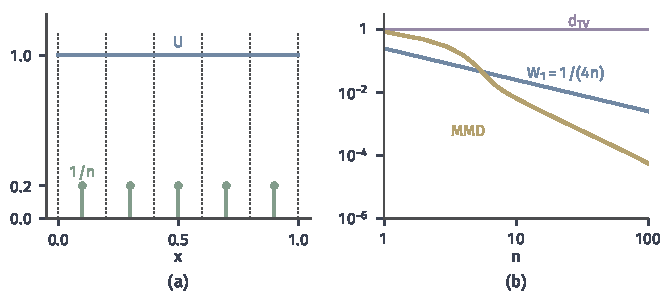
\includegraphics[width=112mm]{figures/07-probability/04-distribution-analysis/matplotlib/dcomp-lattice-metrics/figure.pdf}
 \caption{格点均匀分布逼近$\operatorname{Unif}(0,1)$。(a)$n=5$：绿色竖线是格点上的质量$1/n$，蓝线是$U$的密度，深灰点线是小区间的分界。(b)双对数坐标下的$d_{\mathrm{TV}}(U_n,U)=1$（紫），$W_1(U_n,U)=1/(4n)$（蓝），$\sigma=0.1$高斯核的$\operatorname{MMD}(U_n,U)$（黄，由式~\eqref{eq:dcomp-mmd-kernel}的三个核期望计算）。}
 \label{fig:dcomp-lattice-metrics}
\end{BookInlineFigure}

\subsection{Wasserstein收敛}
\label{sec:dcomp-wasserstein-convergence}

上一小节的格点例子中，$W_1\to0$与弱收敛同时成立。第~\ref{sec:dcomp-tail}节的$P_n=(1-\tfrac1n)\delta_0+\tfrac1n\delta_n$弱收敛到$\delta_0$（对有界连续$f$，$\int f\,\mathrm{d}P_n$与$f(0)$之差是$(f(n)-f(0))/n$，趋于零），$W_1(P_n,\delta_0)$却恒为$1$。差别在于一阶矩：$P_n$的均值恒为$1$，不收敛到$0$。下面的定理说明，这正是两者之间的全部差别。

\begin{theorem}[Wasserstein收敛的刻画]
\label{thm:dcomp-wasserstein-convergence}
设$(E,d)$是Polish空间，$1\leq p<\infty$，$\mu_n,\mu\in\mathcal{P}_p(E)$，$x_0\in E$。则$W_p(\mu_n,\mu)\to0$当且仅当
\begin{equation}
 \mu_n\xrightarrow{\mathrm{w}}\mu\quad\text{且}\quad\int d(x,x_0)^{p}\,\mu_n(\mathrm{d}x)\to\int d(x,x_0)^{p}\,\mu(\mathrm{d}x) .
 \label{eq:dcomp-wasserstein-convergence}
\end{equation}
\end{theorem}

下面证明“仅当”。“当”的方向需要从弱收敛与矩收敛出发构造代价趋于零的耦合，要用到$p$阶矩的一致可积与紧集上的逼近，篇幅较长，读者可查阅~\scite{math-villani2009transport}。

\begin{proof}[“仅当”的证明]
对每个$n$取耦合$\pi_n\in\Pi(\mu_n,\mu)$，使其成本不超过$W_p^{p}(\mu_n,\mu)+1/n$，并设随机变量对$(X_n,X)$服从$\pi_n$（每个$n$用各自的概率空间）。于是
\[
 \varepsilon_n=\bigl(\mathbb{E}\,d(X_n,X)^{p}\bigr)^{1/p}\to0 .
\]

\emph{弱收敛。}设$f$有界且Lipschitz，常数为$L$。由Lyapunov不等式$\mathbb{E}\,d(X_n,X)\leq\varepsilon_n$，
\[
 \Bigl\lvert\int f\,\mathrm{d}\mu_n-\int f\,\mathrm{d}\mu\Bigr\rvert\leq\mathbb{E}\bigl\lvert f(X_n)-f(X)\bigr\rvert\leq L\,\varepsilon_n\to0 .
\]
由Portmanteau定理的有界Lipschitz判据，$\mu_n\xrightarrow{\mathrm{w}}\mu$。

\emph{矩的收敛。}由三角不等式$d(X_n,x_0)\leq d(X_n,X)+d(X,x_0)$与$L^{p}$范数的Minkowski不等式，
\[
 \bigl(\mathbb{E}\,d(X_n,x_0)^{p}\bigr)^{1/p}\leq\varepsilon_n+\bigl(\mathbb{E}\,d(X,x_0)^{p}\bigr)^{1/p} .
\]
交换$X_n$与$X$的角色得到反向不等式，所以两个$p$阶矩的$p$次根之差不超过$\varepsilon_n$，趋于零。
\end{proof}

定理给出了一个清楚的分工：弱收敛管住质量在有界范围内的摆放，矩收敛管住远处有多少质量。第~\ref{sec:dcomp-tail}节的$R_n=(1-n^{-2})\delta_0+n^{-2}\delta_n$是一个检验：它弱收敛到$\delta_0$，一阶矩$1/n\to0$，二阶矩恒为$1$，所以$W_1\to0$而$W_2\not\to0$，与图~\ref{fig:dcomp-far-mass}(b)一致。阶数$p$越高，对远处质量的要求越严。

\paragraph{分布收敛不是取值收敛}
$W_p(\mu_n,\mu)\to0$说的是存在代价越来越小的耦合，而不是某个已经给定的联合实现中的误差变小。设$X\sim\mathcal{N}(0,1)$，$X'$是它的独立副本。$X'$与$X$同分布，$W_p(P_{X'},P_X)=0$，最优耦合是让两者相等。可是在已经给定的独立实现中，
\[
 \mathbb{E}\bigl[(X'-X)^{2}\bigr]=\operatorname{Var}(X')+\operatorname{Var}(X)=2 .
\]
把$X'$换成序列$X_n=X'$（每个$n$都相同），就有$W_2(P_{X_n},P_X)=0$对一切$n$成立，而$\mathbb{E}\lvert X_n-X\rvert^{2}=2$不趋于零。图~\ref{fig:dcomp-coupling-realization}用$300$个模拟点（种子$717$）对比这两种耦合，独立实现的样本平均平方差约为$1.94$。Wasserstein距离只是一个关于分布的结论，不能反推原有共同实现中的$L^{p}$误差；后者是第~\ref{chap:random-variable-convergence}章的$L^{p}$收敛，它要求$X_n$与$X$在同一概率空间上逐点接近。

\begin{BookInlineFigure}
 \centering
 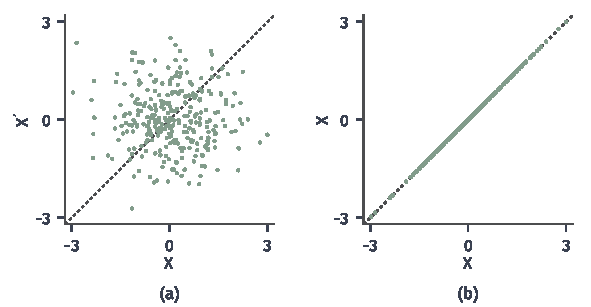
\includegraphics[width=100mm]{figures/07-probability/04-distribution-analysis/matplotlib/dcomp-coupling-realization/figure.pdf}
 \caption{$\mathcal{N}(0,1)$与自身的两种耦合，各$300$个模拟点（绿），种子$717$；深灰点线是$y=x$。(a)独立副本$(X,X')$，$\mathbb{E}(X-X')^{2}=2$，样本值约$1.94$。(b)恒等耦合$(X,X)$，成本为$0=W_2^{2}$。}
 \label{fig:dcomp-coupling-realization}
\end{BookInlineFigure}

\subsection{MMD收敛}
\label{sec:dcomp-mmd-convergence}

特征核保证$\operatorname{MMD}_k(P,Q)=0$当且仅当$P=Q$。一列分布的MMD趋于零是否等价于弱收敛，是另一回事：零点的辨识只涉及单个分布对，收敛还要求比较量不让质量悄悄跑到无穷远，也不对微小平移过度敏感。对$\mathbb{R}^{d}$上固定带宽的高斯核，两件事都成立。

\begin{theorem}[高斯核MMD刻画弱收敛]
\label{thm:dcomp-mmd-weak}
设$\sigma>0$，$k_\sigma$是$\mathbb{R}^{d}$上的高斯核，$P_n,P$是$\mathbb{R}^{d}$上的概率分布。则
\begin{equation}
 \operatorname{MMD}_{k_\sigma}(P_n,P)\to0\quad\Longleftrightarrow\quad P_n\xrightarrow{\mathrm{w}}P .
 \label{eq:dcomp-mmd-weak}
\end{equation}
\end{theorem}

\begin{proof}
\emph{弱收敛推出MMD趋于零。}取相互独立的$\bm{X}_n,\bm{X}_n'\sim P_n$与$\bm{X},\bm{X}'\sim P$。由第~\ref{chap:weak-convergence-of-distributions}章独立分量的联合极限，$(\bm{X}_n,\bm{X}_n')$与$(\bm{X}_n,\bm{X})$都依分布收敛到$(\bm{X},\bm{X}')$。$k_\sigma$在$\mathbb{R}^{d}\times\mathbb{R}^{d}$上有界连续，所以式~\eqref{eq:dcomp-mmd-kernel}中的三项分别趋于$\mathbb{E}[k_\sigma(\bm{X},\bm{X}')]$的$1$倍、$2$倍与$1$倍，和趋于零。

\emph{MMD趋于零推出胎紧。}记$\phi_n,\phi$为特征函数，$\lambda_\sigma$与$\gamma_\tau$分别为$\mathcal{N}(\bm{0},\sigma^{-2}\bm{I})$与$\mathcal{N}(\bm{0},\tau\bm{I})$的密度。令
\[
 h_\tau(\bm{x})=\exp\Bigl(-\frac{\tau}{2}\lVert\bm{x}\rVert_2^{2}\Bigr) .
\]
它是$\mathcal{N}(\bm{0},\tau\bm{I})$的特征函数，由Fubini定理，
\[
 \mathbb{E}_{P_n}[h_\tau]=\int\phi_n(\bm{\omega})\,\gamma_\tau(\bm{\omega})\,\mathrm{d}\bm{\omega} .
\]
于是，由Cauchy--Schwarz不等式与式~\eqref{eq:dcomp-mmd-spectral}，
\[
 \begin{aligned}
 \bigl\lvert\mathbb{E}_{P_n}[h_\tau]-\mathbb{E}_{P}[h_\tau]\bigr\rvert&\leq\int\lvert\phi_n-\phi\rvert\frac{\gamma_\tau}{\lambda_\sigma}\lambda_\sigma\,\mathrm{d}\bm{\omega}\\
 &\leq\operatorname{MMD}_{k_\sigma}(P_n,P)\Bigl(\int\frac{\gamma_\tau^{2}}{\lambda_\sigma}\,\mathrm{d}\bm{\omega}\Bigr)^{1/2} .
 \end{aligned}
\]
$\gamma_\tau^{2}/\lambda_\sigma$正比于$\exp(-(\tau^{-1}-\sigma^{2}/2)\lVert\bm{\omega}\rVert_2^{2})$，当$\tau<2/\sigma^{2}$时可积。所以对这样的$\tau$，$\mathbb{E}_{P_n}[h_\tau]\to\mathbb{E}_{P}[h_\tau]$。

任给$\varepsilon>0$。$\tau\downarrow0$时$h_\tau\uparrow1$，由单调收敛定理可取$\tau<2/\sigma^{2}$使$1-\mathbb{E}_{P}[h_\tau]<\varepsilon$，再取$N$使$n\geq N$时$1-\mathbb{E}_{P_n}[h_\tau]<2\varepsilon$。取$r$使$\mathrm{e}^{-\tau r^{2}/2}\leq\tfrac12$。在$\{\lVert\bm{x}\rVert_2>r\}$上$1-h_\tau\geq\tfrac12$，由Markov不等式，
\[
 P_n\bigl(\lVert\bm{X}\rVert_2>r\bigr)\leq2\bigl(1-\mathbb{E}_{P_n}[h_\tau]\bigr)<4\varepsilon,\qquad n\geq N .
\]
前$N-1$个分布各自胎紧，增大$r$即可一并照顾，所以$\{P_n\}$胎紧。

\emph{子列的极限只能是$P$。}设某个子列$P_{n_j}\xrightarrow{\mathrm{w}}R$。由连续性定理，$\phi_{n_j}\to\phi_R$逐点成立，并且都以$1$为界，由控制收敛定理，$\phi_{n_j}$在$L^{2}(\Lambda_\sigma)$中收敛到$\phi_R$。又由式~\eqref{eq:dcomp-mmd-spectral}，$\phi_{n_j}$在$L^{2}(\Lambda_\sigma)$中到$\phi$的距离就是MMD，趋于零。由$L^{2}(\Lambda_\sigma)$中的三角不等式，$\phi_R=\phi$在$\Lambda_\sigma$几乎处处成立。与定理~\ref{thm:dcomp-gauss-characteristic}的论证相同，$R=P$。由第~\ref{chap:weak-convergence-of-distributions}章的子列原则，$P_n\xrightarrow{\mathrm{w}}P$。
\end{proof}

证明里高斯核起了两个作用。谱权重$\Lambda_\sigma$处处为正，保证极限唯一；它的尾部比$\gamma_\tau^{2}$的尾部衰减得慢，使原点附近的特征函数，也就是“质量是否跑远”的信息，能被MMD控制住。

\paragraph{结论的边界}
高斯核MMD刻画的是弱收敛，不多也不少。它不附带矩的收敛：$P_n=(1-\tfrac1n)\delta_0+\tfrac1n\delta_n$弱收敛到$\delta_0$，所以MMD趋于零（图~\ref{fig:dcomp-far-mass}(a)），均值却恒为$1$。要控制无界函数，仍需第~\ref{sec:dcomp-tail}节的尾部条件。

这个刻画也不能推广到所有特征核。在高斯核上加一个不连续的部分：令$f=\mathbf{1}_{(0,\infty)}$，
\[
 k(x,y)=k_1(x,y)+f(x)f(y),\qquad x,y\in\mathbb{R} .
\]
两个正定核之和仍是正定核，它有界，可以验证相应的RKHS可分、特征映射可测。由式~\eqref{eq:dcomp-mmd-kernel}，
\[
 \operatorname{MMD}_k^{2}(P,Q)=\operatorname{MMD}_{k_1}^{2}(P,Q)+\bigl(P(X>0)-Q(X>0)\bigr)^{2}\geq\operatorname{MMD}_{k_1}^{2}(P,Q),
\]
所以$k$仍是特征核。可是$\delta_{1/n}\xrightarrow{\mathrm{w}}\delta_0$，而第二项恒为$(1-0)^{2}=1$，$\operatorname{MMD}_k(\delta_{1/n},\delta_0)\geq1$不趋于零。不连续的核截面像示性函数一样对微小平移敏感。所以“MMD收敛等价于弱收敛”须同时核对空间与核的条件，例如核的连续性与有界性，不能只凭特征性得出。
